\subsection{Friday Preparation}

The day before the criterium, the \pbproleref{role:lead_org} should ensure the crit course is swept and otherwise cleaned up,
either themselves or with assistance from \pbproleref{role:local_teams}.

Any no-parking signs, barriers, or other materials should be deployed (following the guidance and regulations of the local police and highway department).

The \pbproleref{role:lead_org} should have contracted a towing company to clear the crit course overnight.

\begin{marginfigure}
  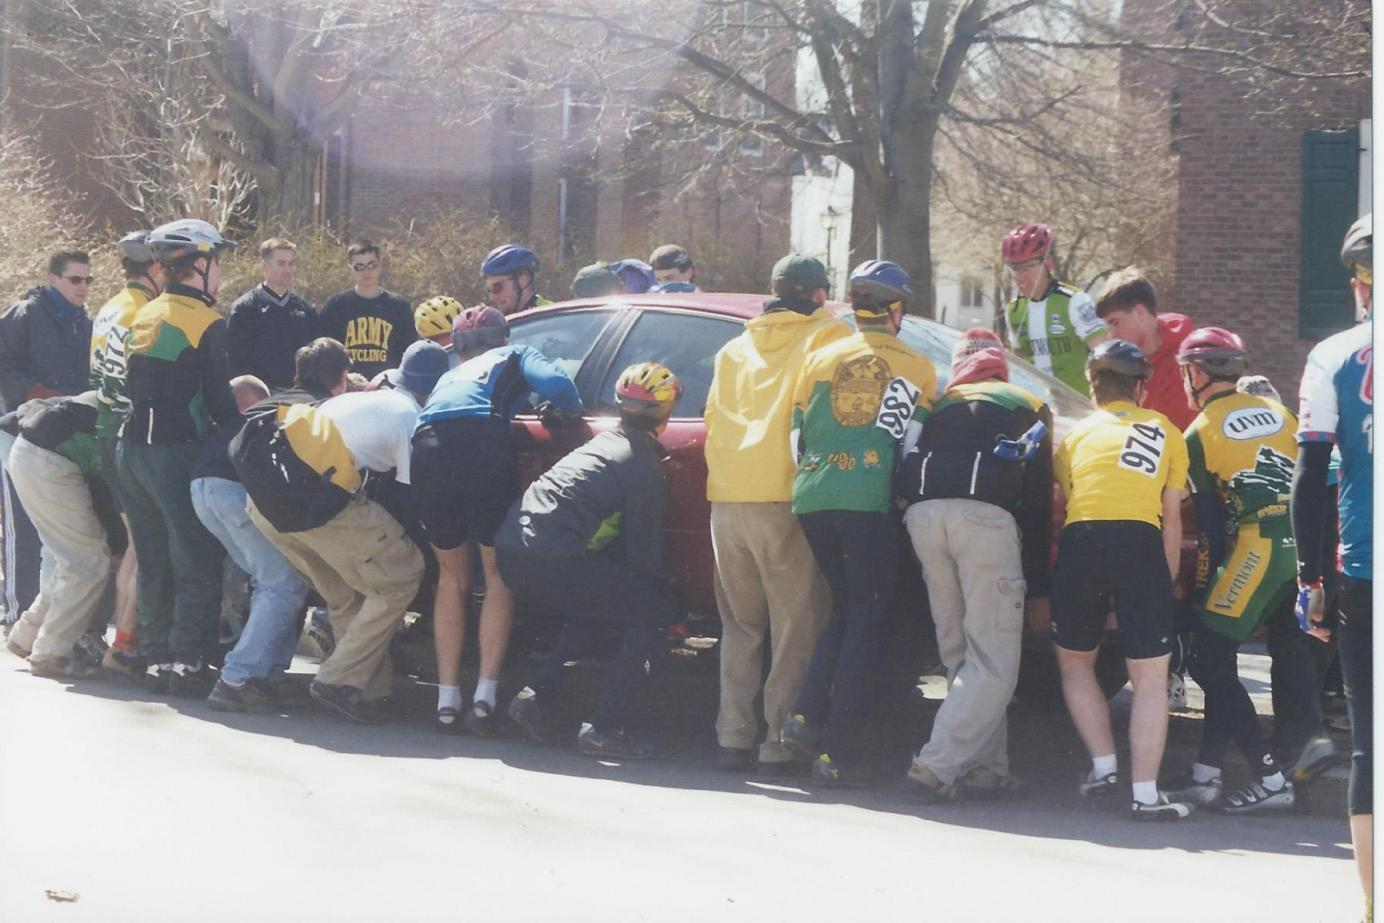
\includegraphics{dartmouth_car.jpg}
  \caption[Students moving a car off a criterium course]{
            Students moving a car off of the Darmouth criterium course
            when towing services were unavailable.\\
            Credit: Alan Atwood}
  \labfig{dartmouth_car}
\end{marginfigure}

The \pbproleref{role:primary_promoter} should call the towing company the night before the race to ensure they are still planning to clear the course -
otherwise you may have to resort to drastic measures (\reffig{dartmouth_car}) to clear the course in the morning!
